\chapter{Technische Grundlagen}

\section{Virtualisierung und paravirtualisierte Geräte}

Virtuelle Maschinen (VMs) ermöglichen das Ausführen eines Betriebssystems in einer isolierten Umgebung, ohne dass dieses direkt auf physische Hardware zugreift. Aus Sicht des Gasts erscheint die Umgebung wie ein vollständiger Rechner. Tatsächlich werden CPU-Ausführung und Gerätezugriffe durch eine Virtualisierungsschicht kontrolliert und bereitgestellt.

\subsection{Host, Gast und Hypervisor}

Die physische Maschine wird als Host bezeichnet, das darin ausgeführte Betriebssystem als Gast. Die Virtualisierungskomponente, die den Gast ausführt und die virtuelle Hardware bereitstellt, wird meist als Hypervisor bzw. Virtual Machine Monitor (VMM) beschrieben, für diese Arbeit ist das QEMU. Im Linux-Umfeld stellt KVM (Kernel-based Virtual Machine) die Hypervisor-Funktionalität im Kernel bereit. VMs werden dabei als Prozesse im Host-System umgesetzt und erhalten „privatisierte“ virtuelle Hardware.\\

In der Praxis kommen unterschiedliche Host-Umgebungen vor \cite{ibm_hypervisor_2024}:

\begin{itemize}
 \item In einer Ubuntu-Umgebung ist KVM eine typische Basis für Virtualisierung.
 \item WSL2 nutzt Virtualisierung und basiert auf einem Subset der Hyper-V-Architektur.
\end{itemize}

Für diese Arbeit ist jedoch wichtig, dass das \texttt{Bare-Metal}-Betriebssystem (D3OS) als Gast in einer VM läuft, und die I/O-Geräte werden durch den VMM bereitgestellt.

\subsection{Gerätemodelle}

Damit ein Gast I/O durchführen kann (z. B. Grafik, Audio), muss der VMM entsprechende Geräte anbieten. Grundsätzlich lassen sich drei Ansätze unterscheiden \cite{redhat_virt_guide_6}:

\begin{enumerate}
 \item \textbf{Emulation:} klassischer Hardware: Der VMM emuliert bekannte Geräte. Das ist kompatibel, kann aber einen höheren Overhead verursachen, da Gerätefunktionen vollständig nachgebildet werden müssen.
 \item \textbf{Passthrough:} Ein reales Gerät wird direkt an den Gast durchgereicht. Dies bietet hohe Nähe zur Hardware, aber höhere Anforderungen an Plattform und Setup und für viele Entwicklungsumgebungen unpraktisch.
 \item \textbf{Paravirtualisierung:} Gast und VMM nutzen ein speziell für Virtualisierung entworfenes Geräteinterface, um Emulationsaufwand zu reduzieren.
\end{enumerate}

Für diese Arbeit ist der dritte Ansatz zentral: VirtIO-Geräte sind paravirtualisierte Geräte, die explizit darauf ausgelegt sind, effizient virtualisiert bzw. emuliert zu werden und daher als empfohlene Gerätemodelle in VMs gelten.


\section{VirtIO-Architektur}

VirtIO ist ein standardisiertes Modell für paravirtualisierte Geräte, das die Aufgaben zwischen Gast und Host bewusst trennt. Im Gast läuft der Treiber (Frontend) als Teil des Betriebssystems, im Host/Hypervisor läuft die Geräteimplementierung (Backend). Beide Seiten kommunizieren nicht über „klassische“ emulierte Register- und Datenpfade historischer Hardware, sondern über ein vereinfachtes, für Virtualisierung optimiertes Protokoll.\\
\\
Der zentrale Kommunikationsmechanismus sind dabei Virtqueues. Das sind im Gast-Speicher abgelegte Warteschlangenstrukturen, auf die Treiber und Gerät zugreifen. Der Treiber hinterlegt Anfragen in Form von Speicherpuffern, die anschließend vom Backend verarbeitet werden. Die Rückmeldung der Ergebnisse erfolgt über dieselben Datenstrukturen, was die Effizienz häufiger Datentransfers maßgeblich steigert \cite{RedHatvirtqueues}.

\begin{figure}[H]
  \centering
  \captionsetup{justification=centering}
  \begin{subfigure}[b]{0.65\textwidth}
    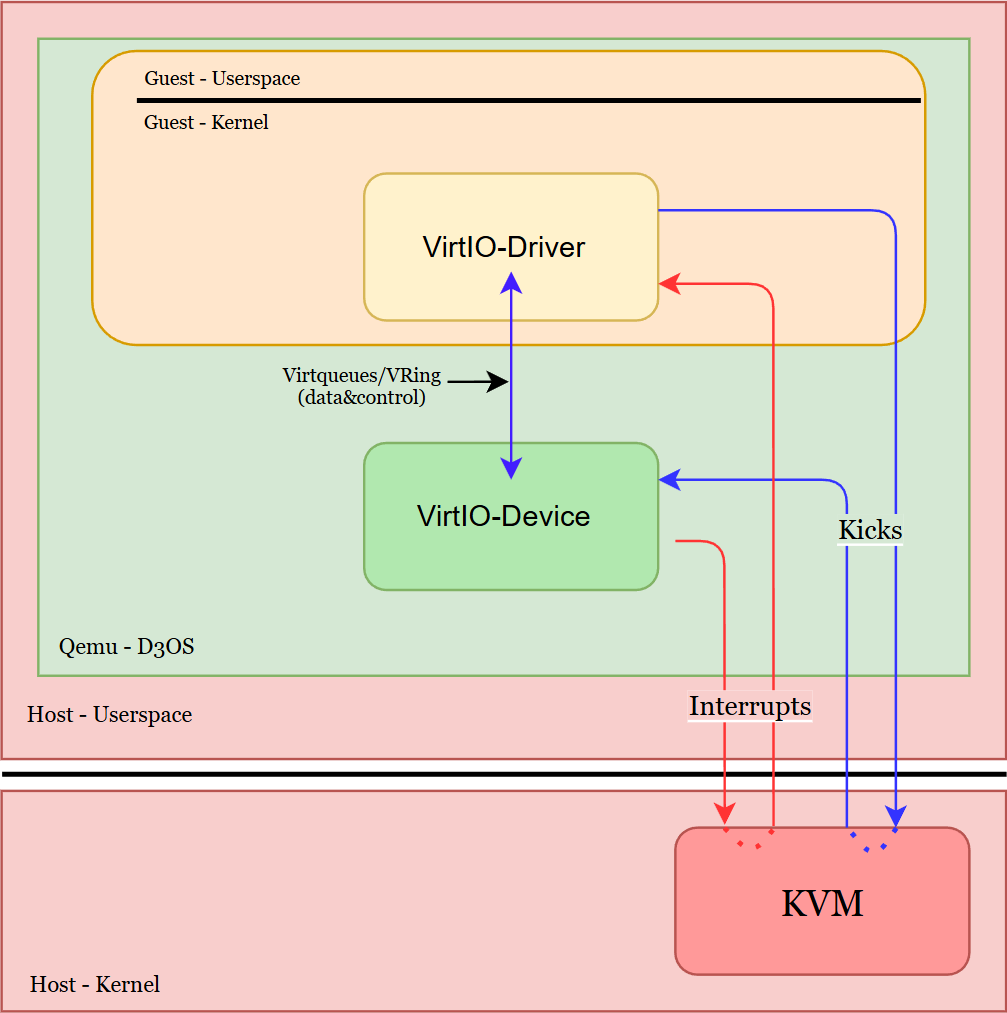
\includegraphics[width=1.0\linewidth]{img/virtio}
  \end{subfigure}
  \caption{Interaktion zwischen VirtIO-Treiber und Gerät\\
   (eigene Darstellung nach \cite{OracleVhost})}
  \label{grafik_1}
\end{figure}


\subsection{VirtIO-Geräte}

VirtIO-Geräte sind virtuelle Peripheriegeräte, die eine virtuelle Maschine (z. B. in QEMU) dem Gastbetriebssystem zur Verfügung stellt. Statt eine konkrete reale Hardware nachzuahmen, bieten diese Geräte eine standardisierte VirtIO-Schnittstelle. Damit das Betriebssystem diese Geräte nutzen kann, braucht es passende VirtIO-Treiber, die das Gerät initialisieren, konfigurieren und I/O-Anfragen über Virtqueues abwickeln.\\
\\
Das VirtIO-Modell ist so definiert, dass es über unterschiedliche „Transports“ bereitgestellt werden kann. Die Transports, welche unterstützt werden sind:

\begin{itemize}
 \item VirtIO over MMIO: Das Gerät stellt Registerbereiche im Memory-Mapped-I/O bereit, der Treiber greift über MMIO auf Status/Features/Queue-Setup zu.
 \item VirtIO over PCI: Das Gerät erscheint als PCI-Gerät und wird über PCI-Mechanismen entdeckt/konfiguriert (häufig bei x86/QEMU).
 \item VirtIO over CCW (s390): Spezielle Transportform für IBM s390-Umgebungen.
\end{itemize}

Bei der in dieser Arbeit behandelten Implementation wird VirtIO over PCI verwendet, da es sich bei D3OS um ein x86 Betriebssystem handelt, welches in QEMU läuft.\\
\\
Unabhängig vom Transport besitzen VirtIO-Geräte wiederkehrende Kernbestandteile, die jeder Treiber bedienen muss \cite{RedHatOverview}:

\subsubsection{Gerätestatus (Device Status)}
Das Statusfeld bildet den Lebenszyklus der Initialisierung ab. Der Treiber bestätigt zunächst, dass er das Gerät erkannt hat, signalisiert dann, dass ein Treiber geladen ist, handelt Features aus und markiert am Ende, dass das Gerät betriebsbereit ist. Tritt ein Fehler auf, können sowohl der Treiber als auch das Gerät einen Fehlerzustand signalisieren. In einem solchen Fall ist in der Regel ein Zurücksetzen der virtuellen Geräteschnittstelle erforderlich, um alle Register und Warteschlangen in einen sauberen Ausgangszustand zu versetzen.
Praktisch ist der Status damit ein Handshake, der verhindert, dass Gerät und Treiber in falscher Reihenfolge arbeiten.

\subsubsection{Feature-Bits (Feature Negotiation)}
VirtIO-Geräte veröffentlichen eine Menge an Fähigkeiten als Bitmaske. Der Treiber wählt daraus die Teilmenge, die er unterstützt und aktivieren möchte. Diese Aushandlung stellt die Kompatibilität zwischen verschiedenen Implementierungsständen sicher. Sie ermöglicht es, Geräte um neue Funktionen zu erweitern, ohne die Lauffähigkeit älterer Treiber zu beeinträchtigen, sofern diese lediglich die ihnen bekannten Feature-Bits verarbeiten.

\subsubsection{Benachrichtigungen (Notifications)}
Sobald der Treiber neue Arbeit in eine Virtqueue gestellt hat, muss das Gerät davon erfahren, z. B. über ein „Notify/Kick“. Umgekehrt signalisiert das Gerät dem Treiber erledigte Arbeit typischerweise über Interrupts (oder der Treiber pollt). In einem Kernel-Design wird häufig der Interrupt nur als „Wecksignal“ genutzt, während die eigentliche Verarbeitung außerhalb des Interrupt-Kontextes erfolgt.

\subsubsection{Gerätekonfigurationsbereich (Device Configuration)}
Zusätzlich zu generischen Strukturen besitzt jedes VirtIO-Gerät einen gerätespezifischen Konfigurationsbereich. Dort stehen Parameter, die für die Nutzung des Geräts relevant sind wie z.B. Eigenschaften der virtuellen Hardware. Treiber lesen diese Werte typischerweise bei der Initialisierung und bei Konfigurationsänderungen.

\subsubsection{Virtqueues}
Virtqueues sind das Transportmittel für I/O-Anfragen und Antworten. Ein Gerät kann mehrere Queues besitzen (z. B. getrennte Queues für Control und Datenpfade). Die genaue Anzahl und Bedeutung hängt vom Gerätetyp ab.

\subsection{Virtqueues}

Das zentrale Element der Datenübertragung zwischen Gast (Treiber) und Host (Device) ist die Virtqueue. Um den Overhead von Kontextwechseln bei der Virtualisierung zu minimieren, setzt VirtIO auf Shared Memory in Kombination mit Direct Memory Access (DMA).\\
Anstatt Daten ineffizient Register für Register durch die CPU zu schleusen, nutzen Treiber und Gerät gemeinsam zugreifbare Speicherstrukturen, um lediglich Metadaten (Deskriptoren) auszutauschen. Diese Deskriptoren verweisen auf physische Speicheradressen im Gastsystem. Das Gerät verarbeitet die eigentlichen Nutzdaten anschließend selbstständig per DMA-Zugriff, ohne dass die Gast-CPU für den Datentransfer belastet wird.

Die VirtIO-Spezifikation kennt dabei zwei Formate für Virtqueues:

\begin{itemize}
 \item \textbf{Split Virtqueue:} klassisches, weit verbreitetes Layout mit drei getrennten Bereichen (Descriptor Table, Avail Ring, Used Ring). Es ist vergleichsweise einfach zu implementieren und zu debuggen.
 \item \textbf{Packed Virtqueue:} moderneres Layout (VirtIO 1.1), das die zuvor getrennten Strukturen stärker zusammenführt und dadurch weniger Speicherzugriffe, weniger Cache-Contention und (bei echter Hardware) weniger PCI-Transaktionen verursacht.
\end{itemize}

Da der in dieser Arbeit eingebundene Treiber-Stack auf Split Queues basiert, wird im Folgenden zunächst dieses Format detailliert erläutert. Packed Queues werden anschließend kurz eingeordnet.

\subsubsection{Split Virtqueue}

Eine Split Virtqueue besteht aus drei Speicherbereichen, die im Gast-Speicher liegen und von Treiber und Gerät gemeinsam genutzt werden. Eine wichtige Eigenschaft ist dabei, dass jeder dieser Bereiche im Normalfall nur von einer Seite beschreibbar ist (Treiber oder Gerät), was Datenrennen reduziert und das Design vereinfacht.

Die drei Bestandteile sind \cite{OASISVirtio12}:

\begin{enumerate}
 \item Descriptor Table (Descriptor Area)
 \item Available Ring (Driver Area/Avail)
 \item Used Ring (Device Area/Used)
\end{enumerate}

Zusätzlich hat jede Queue eine Queue Size (maximale Anzahl gleichzeitig „in flight“ befindlicher Puffer/Requests). Außerdem müssen die einzelnen Teile physisch zusammenhängend im Gast-Speicher liegen und Alignment-Anforderungen erfüllen \cite{RedHatvirtqueues}.

\subsubsection{Descriptor Table}

Die Deskriptortabelle fungiert als das Inhaltsverzeichnis für die eigentlichen Datenpuffer. Sie ist ein Array von Deskriptoren, wobei jeder Eintrag einen Speicherbereich im Adressraum des Gasts beschreibt. Ein einzelner Deskriptor besteht dabei aus vier Kernelementen:

\begin{enumerate}
 \item Address: Die physische 64-Bit-Startadresse des Puffers (GPA - Guest Physical Address).
 \item Length: Die Größe des Puffers in Bytes.
 \item Flags: Steuerflags, die z.B. die Zugriffsrichtung regeln (\code{VIRTIO\_DESC\_F\_WRITE}). Ist dieses Flag gesetzt, darf das Gerät in den Puffer schreiben (z. B. für den Empfang von Netzwerkpaketen), andernfalls ist der Puffer für das Gerät "Read-Only" (z. B. beim Senden).
 \item Next: Ein Index-Verweis auf einen weiteren Deskriptor.
\end{enumerate}

Das Next-Feld und das korrespondierende Flag \code{VIRTIO\_DESC\_F\_WRITE} sind essenziell für das Chaining-Konzept. Da I/O-Anfragen oft aus mehreren Fragmenten bestehen (z. B. einem Protocol-Header und den eigentlichen Nutzdaten), erlaubt VirtIO das Verketten mehrerer Deskriptoren zu einer logischen Einheit. Für das Gerät erscheint eine solche Kette wie ein einziger logischer Puffer, obwohl die Daten physisch fragmentiert im RAM liegen können. Dies reduziert die Notwendigkeit für teure memcpy-Operationen im Gastsystem drastisch.

\subsubsection{Available Ring}

Während die Deskriptortabelle nur die Speicherbereiche definiert, regelt der Available Ring den Besitzübergang dieser Puffer vom Treiber an das Gerät. Er ist der Mechanismus, mit dem der Treiber dem Gerät mitteilt, dass der Puffer vorbereitet wurde und nun vom Gerät verarbeitet werden darf.\\
\\
Der Ring ist als Ringpuffer implementiert, der Indizes enthält, die auf die Köpfe (Heads) von Deskriptorketten in der Deskriptortabelle verweisen. Der Ablauf ist dabei wie folgt:

\begin{enumerate}
 \item Der Treiber füllt freie Deskriptoren mit Pufferinformationen.
 \item Er schreibt den Index des ersten Deskriptors (Head Index) in das nächste freie Slot des Available Rings.
 \item Er inkrementiert den idx-Zeiger des Rings, um dem Gerät zu signalisieren, dass neue Arbeit vorliegt.
\end{enumerate}

Ein entscheidender Aspekt ist hier die Trennung von Daten und Signalisierung. Das bloße Eintragen in den Ring löst noch keine Verarbeitung aus. Erst durch einen expliziten "Kick" (in der Regel ein PIO-Write auf ein Doorbell-Register) wird der Hypervisor/das Gerät benachrichtigt. Um die Anzahl dieser teuren VM-Exits zu reduzieren, unterstützt VirtIO Mechanismen zur Event-Unterdrückung (\code{VIRTIO\_F\_EVENT\_IDX}), bei denen das Gerät dem Treiber mitteilen kann, erst nach einer bestimmten Anzahl neuer Aufträge wieder geweckt zu werden.

\subsubsection{Used Ring}

Der Used Ring ist das Gegenstück zum Available Ring und wird primär vom Gerät beschrieben. Hier trägt das Gerät die Indizes der Deskriptorketten ein, deren Verarbeitung abgeschlossen ist. Sobald ein Eintrag im Used Ring erscheint, geht der Besitz des zugehörigen Speichers wieder an den Treiber zurück.\\
\\
Ein Eintrag im Used Ring enthält neben dem Index der verarbeiteten Kette auch ein \code{len}-Feld. Dieses gibt an, wie viele Bytes das Gerät tatsächlich in den Puffer geschrieben hat. Dies ist besonders bei variablen Datenmengen (wie Netzwerkpaketen) wichtig ist, da sie oft von der ursprünglichen Puffergröße abweichen.\\
\\
Nach dem Aktualisieren des Used Rings sendet das Gerät typischerweise einen Interrupt an den Gast, um den Treiber über die Fertigstellung zu informieren. Auch hier greifen Mechanismen zur Interrupt-Drosselung, um die CPU-Last im Gastsystem zu schonen, wenn das Aufkommen an I/O-Events sehr hoch ist.

\begin{figure}[H]
  \centering
  \begin{subfigure}[b]{0.95\textwidth}
    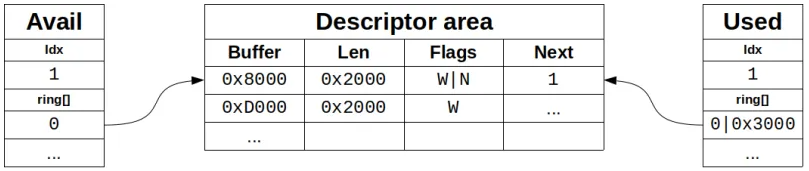
\includegraphics[width=1.0\linewidth]{img/virtqueue}
  \end{subfigure}
  \caption{Der vollständige Zyklus eines Puffers in einer Split Virtqueue \cite{RedHatvirtqueues}}
  \label{grafik_2}
\end{figure}

\subsubsection{Packed Virtqueues}
\label{sssec:packed-virtqueues}

Während das in dieser Arbeit verwendete Split-Layout (Descriptor Table, Available Ring, Used Ring) durch seine robuste Trennung der Speicherbereiche besticht, führt es auf modernen Hardwarearchitekturen zu einem erhöhten Verwaltungsaufwand. Da die drei Bereiche im Speicher verstreut liegen (keine Cache-Lokalität), muss die CPU bzw. das Gerät für eine einzelne I/O-Operation oft auf mehrere, weit voneinander entfernte Cache-Lines zugreifen. Dies erhöht die Anzahl der PCIe-Transaktionen und kann zu sogenannten Cache-Bounces führen \cite{RedHatPacked}.\\

Um diesen Overhead zu adressieren, führt der VirtIO 1.1-Standard das Konzept der Packed Virtqueues ein. Im Gegensatz zum Split-Modell werden hierbei die drei getrennten Strukturen in einer einzigen, linearen Ringstruktur zusammengeführt.\\

Die Funktionsweise unterscheidet sich dabei grundlegend in der Zustandsverwaltung:

\begin{itemize}
 \item Einheitliche Deskriptoren: Jeder Eintrag im Ring enthält sowohl die Daten-Metadaten (Adresse, Länge) als auch den Status des Eintrags. Es gibt keine separaten Indizes für Available oder Used.
 \item Wrap-Counter-Logik: Anstelle eines stetig wachsenden Index wird ein Wrap Counter (Umlaufzähler) verwendet, der als binäres Flag in jedem Deskriptor realisiert ist \cite{RedHatPacked}. Bei jedem Durchlauf des Rings „flippt“ dieses Bit. Treiber und Gerät erkennen anhand dieses Bits, ob ein Eintrag neu bereitgestellt wurde oder noch veraltet ist, ohne auf externe Index-Variablen zugreifen zu müssen.
\end{itemize}

Diese kompaktere Struktur bietet signifikante Vorteile für die Performance, da Treiber und Gerät sequenziell auf denselben Speicherbereich zugreifen, wird die Cache-Nutzung optimiert (bessere Cache-Lokalität) und die Anzahl der notwendigen Speicherzugriffe reduziert.

\subsection{Benachrichtigungssteuerung}

In der Standard-Implementierung können Treiber und Gerät Benachrichtigungen (Interrupts bzw. Kicks) nur pauschal an- oder abschalten. Dies erfolgt über das Flag \code{VRING\_}\allowbreak\code{AVAIL\_F\_NO\_INTERRUPT} im Available Ring sowie \code{VRING\_USED\_F\_NO\_NOTIFY} im Used Ring. Dieser Ansatz ist jedoch oft ineffizient: Schaltet der Treiber Interrupts ab, muss er pollen (Polling), was CPU-Zeit kostet. Lässt er sie an, erzeugt jedes einzelne Paket einen teuren VM-Exit und Kontextwechsel.\\
\\
Um dieses Problem zu lösen, nutzt virtio-drivers das Feature \code{VIRTIO\_F\_EVENT\_IDX}. Dieses Feature ersetzt die pauschalen Flags durch eine genauere Steuerung basierend auf Ring-Indizes. Dabei werden zwei zusätzliche 16-Bit-Felder am Ende der Ring-Strukturen genutzt \cite{RedHatvirtqueues}.

\begin{itemize}
 \item \textbf{used\_event} (im Available Ring): Dieses Feld wird vom Treiber beschrieben und dient der Interrupt-Moderation. Der Treiber hinterlegt hier einen Schwellenwert, der sich auf den Index des Used Rings bezieht. Das Gerät wird durch diesen Mechanismus angewiesen, erst dann einen Interrupt auszulösen, wenn der idx-Zeiger des Used Rings den im used\_event-Feld spezifizierten Wert erreicht.
 \item \textbf{avail\_event} (im Used Ring): Dieses Feld wird vom Gerät verwaltet und steuert die Benachrichtigung durch den Gast (Kick). Das Gerät legt hier fest, wie weit der Treiber den Available Ring füllen darf, bevor eine explizite Benachrichtigung an den Host erforderlich ist. Solange der aktuelle Index des Available Rings den Wert in avail\_event nicht überschreitet, kann der Treiber weitere Deskriptoren bereitstellen, ohne einen teuren VM-Exit zu provozieren.
\end{itemize}

Obwohl diese Mechanismen zur Benachrichtigungsunterdrückung laut Spezifikation lediglich als Optimierung dienen, reduzieren sie den Overhead für die Signalisierung in der Praxis signifikant. Durch die Vermeidung unnötiger Kontextwechsel zwischen Gast und Host wird der I/O-Durchsatz gesteigert, da Benachrichtigungen effizient gebündelt (Batching) verarbeitet werden können \cite[Abschnitt~2.7.7]{OASISVirtio12}.

\section{VirtIO-GPU}

Das VirtIO-GPU-Gerät fungiert als paravirtualisierter Grafikadapter, der dem Gastsystem ermöglicht, grafische Ausgaben zu erzeugen, ohne auf die komplexe Register-Emulation physischer Grafikkarten angewiesen zu sein. In seiner Grundkonfiguration stellt das Gerät einen virtuellen Framebuffer bereit, dessen Inhalte vom Hypervisor (z. B. QEMU) in einem Fenster auf dem Hostsystem dargestellt werden.

\subsubsection{Architektur und Kommunikationskanäle}

Im Gegensatz zu traditionellen Grafikgeräten, die primär über Memory-Mapped I/O (MMIO) Register gesteuert werden, basiert die Steuerung der VirtIO-GPU auf dem Austausch von Kommandostrukturen über Virtqueues. Die Spezifikation definiert hierfür zwei primäre Warteschlangen \cite[Abschnitt~5.7]{OASISVirtio12}:

\begin{enumerate}
 \item \textbf{Control Queue} (Queue 0): Über diesen Kanal werden sämtliche Steuerbefehle gesendet, die den Zustand des Grafikgeräts verändern. Dazu gehören das Erstellen von Ressourcen, das Zuweisen von Speicherbereichen sowie Signalisierungen für Bildschirmaktualisierungen.
 \item \textbf{Cursor Queue} (Queue 1): Diese optionale Queue dient der separaten Steuerung eines Hardware-Mauszeigers. Da diese Funktionalität für die grundlegende Bildausgabe nicht zwingend erforderlich ist, wird sie in vielen Basis-Implementationen vernachlässigt.
\end{enumerate}

\subsubsection{Ressourcen-Management und Framebuffer}

Ein zentrales Konzept der VirtIO-GPU ist die Trennung zwischen der logischen Ressource und dem physischen Backing Store. Eine Ressource ist dabei lediglich ein abstraktes Objekt (identifiziert durch eine Resource-ID), das Metadaten wie Breite, Höhe und Pixelformat (z. B. RGBA, 32-Bit pro Pixel) beschreibt. Damit diese Ressource tatsächlich Daten aufnehmen kann, muss ihr explizit Gast-physischer Speicher zugewiesen werden (Backing). Dieser Speicherbereich fungiert als Framebuffer, in den der Treiber die Farbwerte der einzelnen Pixel schreibt.

\subsubsection{Initialisierungsablauf (2D-Modus)}

Um eine funktionierende Bildausgabe zu etablieren, folgt der Treiber einem definierten Protokoll, das aus vier wesentlichen Phasen besteht. Diese Befehle werden als Anfragestrukturen (Requests) in die Control Queue gestellt und vom Gerät quittiert \cite[Abschnitt~5.7]{OASISVirtio12}:

\begin{enumerate}
 \item Erkennung der Display-Konfiguration (GET\_DISPLAY\_INFO): Zunächst fragt der Treiber die aktuelle Konfiguration des virtuellen Monitors ab. Das Gerät liefert Informationen über unterstützte Auflösungen oder die aktuelle Fenstergröße des Hypervisors zurück. Dies ermöglicht dem Gast, seine interne Auflösung dynamisch anzupassen.
 \item Erstellung der 2D-Ressource (RESOURCE\_CREATE\_2D): Der Treiber weist das Gerät an, eine neue interne Ressource mit einer eindeutigen ID zu erstellen. Hierbei werden das Format (typischerweise B8G8R8A8\_UNORM) sowie die Dimensionen (Breite und Höhe) festgelegt. Zu diesem Zeitpunkt besitzt die Ressource noch keinen Speicherplatz für Bilddaten.
 \item Zuweisung des Speichers (RESOURCE\_ATTACH\_BACKING): Im dritten Schritt verknüpft der Treiber die zuvor erstellte Ressource mit einem physischen Speicherbereich im RAM des Gasts. Der Treiber übergibt hierbei eine Liste von Speicheradressen (Scatter-Gather-Liste), die als Backing Store dienen. Ab diesem Moment kann das Gerät per DMA (Direct Memory Access) auf die Pixeldaten zugreifen, die der Treiber in diesen Speicherbereich schreibt.
 \item Datenübertragung (TRANSFER\_TO\_HOST\_2D): Nachdem der Treiber Pixeldaten in den lokalen Backing-Store geschrieben hat, sendet er diesen Befehl. Er weist das Gerät an, die Daten aus dem Gast-Speicher in die interne Ressource des Hosts (z. B. in den Videospeicher der Host-Grafikkarte) zu kopieren.
 \item Aktivierung der Ausgabe (SET\_SCANOUT): Abschließend wird die Verbindung zwischen der Ressource und dem virtuellen Monitorausgang (Scanout) hergestellt. Durch diesen Befehl wird festgelegt, dass der Inhalt der spezifischen Ressource auf dem Bildschirm dargestellt werden soll.
\end{enumerate}

Um Änderungen sichtbar zu machen, muss jedoch zwingend ein Flush-Befehl (RESOURCE\_FLUSH) gesendet werden, der den Hypervisor anweist, die geänderten Daten aus dem Gastspeicher zu lesen und das Host-Fenster zu aktualisieren.\\
Während dieser 2D-Modus für einfache grafische Oberflächen ausreicht, stößt er bei komplexeren Anwendungen an seine Grenzen: Er erlaubt lediglich den Austausch fertiger Pixeldaten (Dumb Framebuffer), bietet jedoch keine Möglichkeit, die Rechenleistung der Host-GPU für Renderoperationen zu nutzen. Um hardwarebeschleunigtes Rendering zu ermöglichen, erweitert der Standard die Spezifikation um 3D-Funktionalitäten. Die technische Basis hierfür bildet das VirGL-Protokoll, dessen Funktionsweise im folgenden Abschnitt erläutert wird.

\subsection{3D-Beschleunigung und VirGL}

Die Erweiterung des VirtIO-GPU-Standards um 3D-Fähigkeiten (\textbf{virgl}) verfolgt das Ziel, OpenGL oder Vulkan-Befehle vom Gast an den Host durchzureichen, um dessen Hardwarebeschleunigung zu nutzen.\\
\\
Insbesondere für ein eigenständiges Bare-Metal-Betriebssystem wie D3OS stellt dies eine signifikante Hürde dar. Etablierte Systeme (wie Linux) greifen auf komplexe Grafik-Stacks (z. B. Mesa 3D) zurück, die Millionen Zeilen Code umfassen, um High-Level-APIs wie OpenGL oder Vulkan bereitzustellen. Da die Implementierung eines vergleichbaren, vollständigen 3D-Stacks, inklusive Shader, Compiler, Speicherverwaltung und State-Tracker, den Rahmen dieser Bachelorarbeit überschreiten würde, wird in dieser Arbeit kein vollständiger 3D-Grafikstack realisiert. Der Fokus liegt stattdessen auf der Enabling-Technologie: Der Implementierung des Transportmechanismus, der es dem D3OS-Kernel erlaubt, grundlegende 3D-Befehlsketten zu konstruieren und erfolgreich an den Host zu übertragen.\\
\\
Um dies hardwareunabhängig zu ermöglichen, definiert VirGL eine virtuelle 3D-GPU mit einem standardisierten Befehlssatz. Da der Gast nicht wissen kann, welche physische Grafikkarte im Host verbaut ist (z. B. NVIDIA, AMD oder Intel), kann er keine herstellerspezifischen Treiber verwenden. VirGL fungiert hier als Abstraktionsschicht, die stark an die Architektur von Gallium3D (einem Treiber-Framework des Linux-Grafikstacks) angelehnt ist \cite{MesaVirGL}.\\
\\
Funktionsprinzip: Der Gallium-Passthrough Der Datenfluss bei der 3D-Beschleunigung unterscheidet sich fundamental vom 2D-Modus. Anstatt Pixel zu kopieren, serialisiert der Treiber im Gastsystem Grafikbefehle (z. B. „Setze Viewport“, „Lade Shader“, „Zeichne Dreieck“) in einen binären Datenstrom.

\begin{enumerate}
 \item Gast (Frontend): Der Treiber kodiert High-Level-Grafikoperationen in das VirGL-Protokoll. Diese Befehle werden in einen Speicherpuffer geschrieben (Command Buffer).
 \item Transport: Über die Virtqueue (speziell über den Befehl SUBMIT\_3D) wird dieser Puffer an den Host übergeben.
 \item Host (Backend): Auf der Host-Seite läuft eine Komponente (in QEMU typischerweise virglrenderer), die diesen Bytecode entgegennimmt \cite{VirglDecode}. Sie analysiert die Befehle und übersetzt sie in die native Grafik-API des Hosts (z. B. echtes OpenGL). 
\end{enumerate}

\begin{figure}[H]
  \centering
  \begin{subfigure}[b]{0.75\textwidth}
    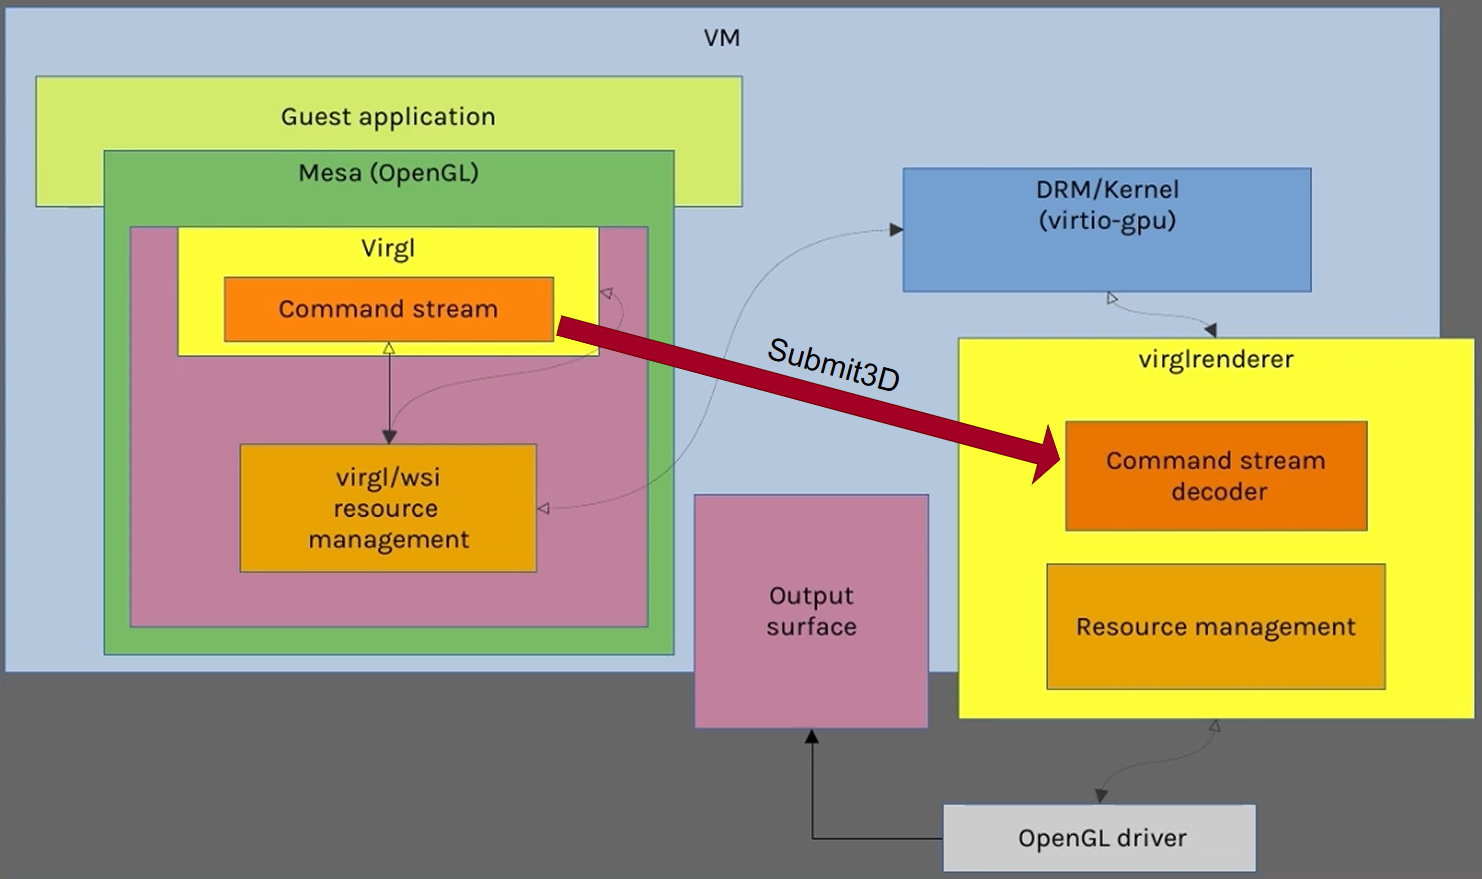
\includegraphics[width=1.0\linewidth]{img/virgl.drawio}
  \end{subfigure}
  \caption{Referenzarchitektur des VirGL-Renderings im Linux-Grafikstack (Mesa) \cite{LVC21F218VirGLSlides}}
  \label{fig:virgl}
\end{figure}

Die in Abbildung 2.3 dargestellte Architektur visualisiert das Zusammenspiel dieser Komponenten in einem Linux-Referenzsystem. Während dort der Mesa 3D-Stack (grüner Block) die Übersetzung der OpenGL-Befehle übernimmt, verdeutlicht die Grafik den Ansatzpunkt der D3OS-Implementierung. Sie ersetzt den gesamten linken Software-Stack (Gast-Applikation und Mesa).\\
Der in Kapitel 4 entwickelte Treiber fungiert direkt als Command Stream Encoder (orange Box im Gast). Anstatt High-Level-APIs bereitzustellen, generiert er die binären Befehlsdaten manuell und übergibt sie an den Transportmechanismus. Für den Host (rechte Seite der Abbildung) ist dieser Unterschied transparent, da der generierte Command-Stream dem Protokollstandard entspricht, verarbeitet der \texttt{virglrenderer} die Befehle identisch, unabhängig davon, ob sie von einem komplexen Grafikstack oder der direkten Treiberimplementierung stammen.\\
\\
Um diesen Mechanismus zu nutzen, führt VirtIO-GPU neue Objekttypen und Kommandos ein, die für das Verständnis der späteren Implementation essenziell sind:

\begin{itemize}
 \item \textbf{Virtuelle Kontexte} (CTX): Im Gegensatz zum globalen Zustand des 2D-Modus kapselt VirGL Zustände in Kontexten. Ein Kontext entspricht isolierten OpenGL-Zuständen. Bevor 3D-Befehle gesendet werden können, muss der Treiber mittels CTX\_CREATE einen Kontext erstellen. Dies ermöglicht es dem Host, mehrere grafische Anwendungen verschiedener VMs sauber zu trennen.
 \item \textbf{3D-Ressourcen}: Ressourcen im 3D-Modus (RESOURCE\_CREATE\_3D) sind mä\-chtiger als ihre 2D-Pendants. Sie besitzen Attribute wie Bind-Flags, die definieren, wie die Ressource genutzt wird (z. B. als Vertex-Buffer, Index-Buffer oder Render-Target). Diese Ressourcen müssen explizit an einen Kontext gebunden werden (CTX\_\allowbreak ATTACH\_RESOURCE), bevor die virtuelle GPU darauf zugreifen kann.
 \item \textbf{Command Submission}: Ein zentraler Bestandteil der 3D-Kommunikation ist die Übermittlung von Befehlen, der Befehl VIRTIO\_GPU\_CMD\_SUBMIT\_3D überträgt dabei den Command-Stream an den Host. Da Rendering asynchron erfolgt, ist hierbei die Synchronisation entscheidend. Mithilfe von Fences kann der Treiber markieren, wann eine bestimmte Befehlsfolge vom Host abgearbeitet wurde, um Race Conditions im Speicherzugriff zu vermeiden.
\end{itemize}

Durch diese Architektur wird VirtIO-GPU von einem einfachen Framebuffer-Gerät zu einer vollwertigen, programmierbaren Grafikpipeline erweitert, die dem Gastsystem erlaubt, komplexe 3D-Szenen hardwarebeschleunigt zu rendern.

\section{VirtIO-Sound}

Das VirtIO-Sound-Gerät (virtio-snd) stellt eine paravirtualisierte Soundkarte bereit, die sowohl die Wiedergabe (Playback) als auch die Aufnahme (Capture) von Audiodaten ermöglicht. Im Gegensatz zu älteren emulierten Standards (wie AC'97 oder Intel HDA), die oft komplexe Register-Interfaces besitzen, setzt VirtIO-Sound konsequent auf den nachrichtenbasierten Austausch über Virtqueues.

\subsection{Architektur und Warteschlangen}

Die Spezifikation definiert für das Sound-Gerät vier spezialisierte Warteschlangen, die unterschiedliche Aspekte der Audiosteuerung und Datenübertragung abdecken \cite[Abschnitt~5.14]{OASISVirtio12}:

\begin{enumerate}
 \item \textbf{Control Queue} (Queue 0): Über diesen Kanal werden administrative Aufgaben abgewickelt. Der Treiber nutzt ihn, um Informationen über verfügbare Anschlüsse (Jacks) und Datenströme (Streams) abzufragen oder um Hardware-Parameter wie die Sample-Rate und das Datenformat zu konfigurieren. Auch Zustandswechsel (Start/Stop von Streams) werden hier initiiert.
 \item \textbf{Event Queue} (Queue 1): Diese Queue dient dem asynchronen Empfang von Benachrichtigungen. Das Gerät informiert den Treiber hierüber beispielsweise, wenn ein Kopfhörer eingesteckt wurde (Jack-Remapping) oder wenn ein abgespielter Audioabschnitt (Period) verarbeitet wurde. Da Audioverarbeitung zeitkritisch ist, ermöglicht diese Trennung von der Control-Queue eine effiziente Ereignisbehandlung.
 \item \textbf{TX Queue} (Transmit/Queue 2): Dies ist der Datenkanal für die Wiedergabe. Der Treiber stellt Puffer mit PCM-Audiodaten (Pulse Code Modulation) in diese Queue. Das Gerät entnimmt die Daten und leitet sie an das Audio-Backend des Hosts weiter.
 \item \textbf{RX Queue} (Receive/Queue 3): Dies ist der Datenkanal für die Aufnahme. Der Treiber stellt hier leere Puffer bereit, die vom Gerät mit Audiodaten (z. B. vom Mikrofon) gefüllt werden.
\end{enumerate}

\begin{figure}[H]
  \centering
  \begin{subfigure}[b]{0.75\textwidth}
    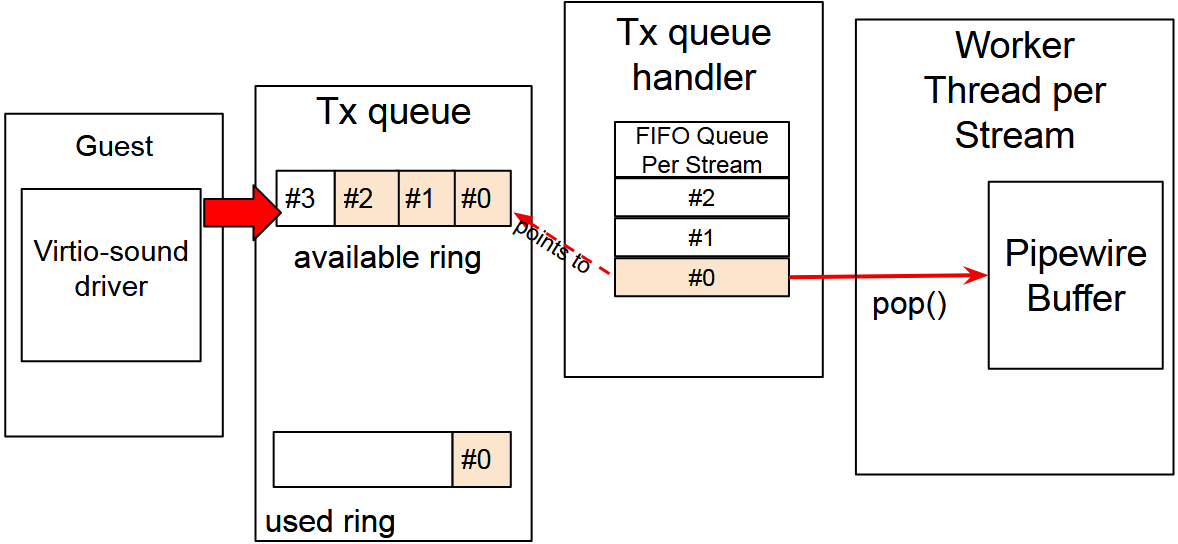
\includegraphics[width=1.0\linewidth]{img/audioqueue}
  \end{subfigure}
  \caption{Datenfluss der VirtIO-Sound TX-Queue (Playback) \cite{FOSDEM2024VirtioSoundSlides}}
  \label{fig:audio}
\end{figure}

Die in Abbildung 2.4 dargestellte Architektur visualisiert den Datenfluss innerhalb der TX Queue während der Audiowiedergabe. Auf der linken Seite platziert der VirtIO-Sound-Treiber des Gastsystems Audiodaten in Form von einzelnen Perioden (hier nummeriert als 0 bis 3) in den Available Ring. Dieser Ring fungiert als geteilter Speicherbereich, über den der Treiber neue Aufgaben ankündigt.\\
Auf der Host-Seite (rechts) überwacht ein Queue Handler diesen Ring. Sobald neue Puffer verfügbar sind, im Diagramm exemplarisch Puffer 0, werden diese entnommen (pop) und verarbeitet. Das Diagramm zeigt hierbei Pipewire als das Audio-Backend des Hosts. Dies repräsentiert eine typische Konfiguration auf modernen Linux-Hostsystemen (wie dem in der Evaluation genutzten Ubuntu 25.10), bei denen der Hypervisor (QEMU) die Audiodaten aus dem Virtqueue direkt an den Pipewire-Soundserver des Hosts weiterleitet, um die Ausgabe zu realisieren.

\subsubsection{Logische Komponenten: Jacks und Streams}

Das Gerätemodell abstrahiert die Audio-Hardware in zwei Hauptkomponenten:

\begin{itemize}
 \item \textbf{Jacks:} Repräsentieren physische Anschlüsse (z. B. Mikrofonbuchse, Line-Out). Sie besitzen Eigenschaften wie Verbindungsstatus und Pin-Belegung.
 \item \textbf{PCM Streams:} Repräsentieren die logischen Datenflüsse für Input oder Output. Ein Stream ist durch Parameter wie Kanalanzahl (Mono/Stereo), Format (z. B. 16-Bit Signed Integer) und Frequenz (Sample Rate) definiert.
\end{itemize}

\subsubsection{Pufferung und Perioden}

Eine Besonderheit der Audioverarbeitung ist die Notwendigkeit eines konstanten Datenflusses, um Aussetzer (Glitches) zu vermeiden. VirtIO-Sound unterteilt den Audiopuffer dazu in logische Abschnitte, sogenannte Perioden. Anstatt einen einzigen riesigen Puffer zu übergeben, zerlegt der Treiber den Datenstrom in periodengroße Blöcke (Chunks). Das Gerät verarbeitet diese Blöcke sequenziell und sendet nach Abschluss einer Periode optional eine Benachrichtigung (Elapsed Period Message) über die Event-Queue. Dies erlaubt dem Treiber, den Füllstand des Puffers präzise zu überwachen und rechtzeitig neue Daten nachzuliefern (Double- oder Ring-Buffering).